\chapter{関連研究}
\label{related_works}

近年、道具や機械、VR上のアバター、そしてインタラクティブな作品といった対象と、人との関係を捉える言葉として、「embodiment」が用いられている。Embodimentの意味は「具現化、身体化」など様々だが、本章では「embodiment」を「身体化」として捉える立場、「一体化」として捉える立場について紹介する。その上で、本研究が着目する「人馬一体」について、「``一体化''としてのembodiment」の立場にあると考えられる、Sydney Felsの提唱したモデルを用いて説明し、本研究の位置付けを明らかにする。

\section{``身体化''としてのembodiment}
「身体化(embodiment)」は心理学や認知科学の領域で、「身体化感覚(sense of embodiment)」を中心として実証的知見が蓄積されている。身体化感覚は、身体に対する所有感(sense of body ownership)、行為主体感(sense of agency)、そして自己位置感覚(sense of self-location)を合わせた感覚として取り扱われることが多い\cite{kilteni2012}。その元となったのは、Gallagherの「ミニマルセルフ」という概念である。「ミニマルセルフ」とは、自我としてみなしうる必要最小限のもののことであり、身体所有感(sense of ownership)、行為主体感(sense of agency)の二つから構成されていると説明される\cite{Gallagher2000}。こうした自己についての説明を実験的に操作・検証可能であることを示したのがBotvinick \& Cohenによるラバーハンド錯覚\cite{BotvinickCohen1998}である。これは、自分の手を衝立の裏に隠し、ラバー製の手を目の前に置いた状態で、両方に同じタイミングで刺激を提示すると、偽物の手を自分の手であるように感じる錯覚である。この報告により、外界の対象への身体所有感の生起が可能であることが示されたとともに、身体所有感研究に関する系統的な手法が探求されることとなった。

VRやロボティクスなどの分野では、「私たちはどこまでを自分の身体として認識(身体化)しうるか?」について、その可能性と限界を探る研究や、そうした知見の応用を提唱する研究へと繋がっている。以下では、身体化感覚における探求や応用について、一例を紹介する。

VRを用いた身体化感覚の研究では、身体の別の部位への動きのマッピングやユーザが同時に操作する身体の数などを操作変数とすることで、新しい心理学研究の可能性を拓くような研究がなされている。例えば近藤ら\cite{Kondo2020}は、右手の親指の動きにVR上の左腕の動きを連動させることで錯覚的な身体所有感(Illusory Ownership)が生じるのかについて検証した。被験者は、右手の親指の動きがVR上での左腕の動きにマッピングされている様子をヘッドマウントディスプレイを介して確認する。実験では、被験者に5分間自由に指先を動かしてもらった後、VR上で左腕のあたりにナイフが突然出現する。このときの皮膚コンダクタンス反応(Skin Conductance Response, SCR)の計測と、身体化感覚(embodiment)に関するアンケートを20人の被験者に行った結果、この手法を通して右手の親指と左腕の結びつき(re-association)は、程度は弱いが誘発できると報告している。また佐々木ら\cite{sasaki2022multisoma}は、VR上で最大4つの身体を制御できるシステムを実装し、複数の身体を制御する際、人間の身体認知がいかに更新されるかについて検討した。実験では3つのタスクを設定し、視線情報、タスクのパフォーマンス、身体化感覚(sense of embodiment)についての主観評価により、これらの身体の認知を評価した。結果、人間は複数の身体を同時に操作することで、それぞれの身体に対して身体所有感(sense of ownership)や運動主体感(sense of agency)を持つことができると報告している。

また、トレーニングを通した身体化感覚の変化を扱う研究も行われている。Kielibaら\cite{kieliba2021robotic}は、ロボットで拡張された親指が人間の運動能力を拡張させることができるかどうか、そしてそれが手の神経表現や機能にどのような影響を与えるのかを調査するため、The Third Thumbというロボットの親指を用いた研究を行った。この親指は、足のつま先で操作することができる。5人の参加者は、5日間にわたってThe Third Thumbを装着し、実験室での使用と日常生活での使用が求められた。通常は両手を使って行うタスクをこの親指を駆使して片手で行い、その器用さ(dexterity)や身体化感覚(sense of embodiment)などの度合いが評価された。トレーニングを経て、認知的負荷が増加した場合や視覚が遮断された場合でも、親指の運動制御、器用さ、そしてThe Third Thumbに対する身体化感覚(sense of embodiment)が向上したと報告している。

さらに、こうした考え方をユーザインターフェースのような道具の操作性について議論するために援用する例も見られる。インターフェース研究者の渡邊は、ユーザインターフェースにおける「透明性」を実現する上で「自己帰属感(sense of ownership)」に着目した\cite{Watanabe2017}。ここで「透明性」とは、道具の使用において、使っている最中にはその道具自体を意識せずに身体の一部になったかのようになり、目的に集中できるようにすることとされている。そして、道具の透明性は「自己帰属感」によってもたらされると考え、マウスカーソルを対象に、ユーザインターフェースにおける自己帰属感を検証する「ダミーカーソル実験」を行った\cite{Watanabe2013}。この実験ではスクリーン上に、マウスと連動して動く通常のカーソルの他に色形状の同じの複数のダミーのカーソルをランダムに動くように同時に提示する。被験者は動きのみでしか自身のカーソルを判別することができない環境になる。そしてこの実験によって、人は動きのみであっても複数のダミーカーソルの中から自身のカーソルを発見できると報告されている。どれが自分のカーソルか判別できることから、人間はカーソルに対しても自己を見出しており、自己帰属感が生起していると主張している。これを踏まえて、ユーザインターフェースにおける自己帰属感を生起するために、操作時の動作とグラフィックの追従性が重要となることを指摘した。

\section{``一体化''としてのembodiment}
ここまで概観したように、「``身体化''としてのembodiment」については、その探究や応用を提示する研究が発展してきた。しかし、これらの議論で前提とされてきた「自己に帰属する他者」という意味でのembodimentのみでは、捉えきれない人と対象との関係があるのではないだろうか。
ここで、embodimentという言葉について原義に立ち返って考えたい。Embodimentは日本語で「身体化、具体化」などと訳されるが、動詞の「embody」についてCambridge Dictionaryで引くと、
\begin{quote}
  \begin{enumerate}
    \item \textit{to represent a quality or an idea exactly} (質や考えを的確に表すこと) 
    \item \textit{to include as part of something} ((何かを)何かの一部として取り込むこと)
  \end{enumerate}
\end{quote}
とある\cite{embody}。ここで指摘したいのは、2つ目の意味からembodimentの原義とは「何かを取り込んで、何かの一部とすること」であり、「人間の一部として対象が帰属しているような状態」のみを指すわけではないということだ。「自己に帰属する他者」という主従関係(=身体化)から自由になって人と他者との関係を捉え直すと、embodimentの研究には「他者に帰属する自己」という関係も捉えられるようになる。このような、自己と他者の主従関係を問わないembodimentを、ここでは「``一体化''としてのembodiment」とする。本節では、そのような立場からembodimentを捉えていると考えられる研究を2つ紹介する。

\subsection{人馬一体感}
心理学研究者の大北らは、ヒトとウマという異種間の間に芽生える一体感である「人馬一体」感について、どのようなプロセスで生じるのか、またそれはどのような感覚なのかを明らかにする目的で、馬術経験者に対するインタビューから概念生成を行った\cite{ohkita2018}。結果、人がウマに対しておこなう「扶助」と呼ばれる非言語シグナルに対して、時間的に接近してウマが行動を変化させたときに、操作主体感といった自己の身体保持感(sense of ownership)の拡張が生じるだけでなく、ウマというヒト(自己)以外のエージェントが協働したことによって「ウマと心が通じ合えた」といった円滑なインタラクション感も得ている可能性が示されたと報告している。このように、自己と他者との関係について、一方的に人に帰属するような他者の観点のみならず、ヒトとウマの間に芽生えた相互学習や、ヒトが対象に対して帰属していくような感覚を通して、一体感が生起することを捉える視点も存在する。

\subsection{Sidney Felsによるembodiment}
\label{Fels_model}
コンピューター工学者のSidney Felsは、「Intimacy and Embodiment: Implications for Art and Technology」\cite{Fels}において、人間と対象との関係性を「embodiment」の観点から4つのカテゴリに分類した。4つの分類とは、以下の通りである。

\begin{quote}
  \begin{enumerate}
    \item the person communicates with the object in a dialogue,
    \item the person embodies the object,
    \item the object communicates with the person, and
    \item the object embodies the person.
  \end{enumerate}
\end{quote}

ここで、後半の2つのカテゴリは、「対象に帰属する人間」という、embodimentにおける``身体化''とは逆の主従関係を捉える区分として特徴的と言える。

Felsは、人と対象との4つの関係のそれぞれで、異なる美的体験をしていると説明する。このようなモデルを用いることで、Fels自身が制作したインタラクティブ作品である《Iamascope》をはじめ、複数の事例に関して人と対象との関係を説明する。その背景には、90年代に演算装置を用いた作品が登場し、鑑賞だけではない作品との関係が生じた中で、芸術表現に科学技術を用いることを特徴づけるものを捉えたいという意図があったと考えられる。

\section{本研究の位置付け}
前節で取り上げた「``一体化''としてのembodiment」は、「自己に帰属する他者」という関係だけでなく、「他者に帰属する自己」という関係を含んでいる。大北らの「人馬一体感」では、ウマとヒトの「協働」の過程に見られる。単にウマがヒトの命令に対して従順になるだけではなく、ヒトがウマの上下運動のリズムを学習するなど、「ウマに帰属するヒト」の関係が見られる。また、Felsのembodimentでは、後ろ2つの区分がまさに「他者に帰属する自己」という関係である。

この観点から本研究は「``一体化''としてのembodiment」の立場に注目し、「対象を帰属させる」と同時に「対象に帰属する」、これら両方が起こる状態として、「人馬一体」という関係性を扱う。本研究の人馬一体とは、自己の抱く目的を直ちに達成できてしまうような扱いやすいものではなく、注意を向ける必要があるような対象との関係の中で芽生えるものである。対象の思うようにいかなさやわかりづらさに向き合い、その振る舞いに注意を向け、それに合わせた身体の動かし方を身につけることで、主観的な一体感が得られるような関係性を指す。こうした関係は、例えば楽器やバイクとのあいだなどにもみられる。

ここでの「人馬一体」感とは、大北らとは用法が異なる。大北らは「人馬一体」感を、自己の身体保持感の拡張と、ヒト以外のエージェントとの協働による「心が通じ合えた」といった円滑なインタラクション感を得る感覚であるとした。そのため、大北らの意味での「人馬一体」は、ヒトと無生物とのあいだには生起しないとしている。対象がヒト以外のエージェントではない本研究での「人馬一体」感は、「心が通じ合えた」という感覚を含まない。しかし、意識的に対応関係を探ったり、それに合わせた行動様式を習得したのち、後から得られる一体感は、「心が通じ合えた」ときに似た喜びとして経験されるのではないか。

では、本研究の「人馬一体」が生起するような関係とは、どのように設計できるのか。それを考えるにあたって、本研究では先のFelsの分類から「人馬一体」を説明する。\ref{Fels_model}節で紹介したFelsの分類は、のちにCostelloら\cite{Costello2005}によって、《Iamascope》の作品体験をより精緻に捉えるための枠組みとして援用され、それぞれ\textit{response}、\textit{control}、\textit{contemplation}、\textit{belonging}と命名された。これら4つの分類について、その詳細を示す(括弧内は筆者訳)。

\textbf{\textit{Response}(応答):}\\
対象に働きかけ、その応答次第で何をするか決める「対話」のような対象との関係を指す。この時は、人と対象とのあいだに一体感は芽生えていない。Felsは、人と対象がこの関係下にあるときに感じる美的体験とは、人が期待していたことに対して予想通りの反応が得られるかどうかにかかっているという。Felsはこの関係下にある状態の例として「コンピュータとそれに初めて触れた人」を挙げ、「なんらかの操作を通して得られた、便利な機能に喜んでいる状態と説明する。

\textbf{\textit{Control}(制御):}\\
人は対象を、自分自身の延長のように感じている。このときに感じる感情的な満足や美的体験とは、操作そのものによってもたらされる。これは例えばピアノの演奏において、「音が出ている」ということだけでなく、自分自身の表現したいことが、不自由なくピアノを通して体現されていると感じるときの、一体感によってもたらされる心地よさが該当する \footnote{「Control」においてFelsは、「自分自身の延長」として経験される感覚であり、またそれが追従性の高いグラフィックによってもたらされると説明する。これは、渡邊がマウスカーソルやスマートフォンに対して用いた「操作時の指とグラフィックの追従性が高い」インターフェースという説明と同等のものであると考えられる。このことからFelsの分類におけるControlは、渡邊の「自己帰属感」と重なる。}。

\textbf{\textit{Contemplation}(熟考):}\\
人が対象からの信号やメッセージについて、内省や熟考することを通じて、感情的になったり美的体験を得る状態を指す。このとき、人が対象に対して働きかけることはない。その具体例として、絵画の鑑賞体験が該当する。

\textbf{\textit{Belonging}(帰属):}\\
この関係は、字面通りに解釈すると理解しづらい。そこで以下では、FelsやCostelloらがこの関係について言及している文章を追うことでこの関係のイメージを捉える。Felsは、次のように説明する。

\begin{quote}
  第4の関係(筆者注: \textit{belonging})では、対象が人を取り込む。この状況では、人は対象が自分を操作できるように、自分が操作することを放棄することで美的感覚を得る。感情的な反応は、服従と帰属によってもたらされる。このタイプの関係では、対象は人を操作できなければならず、人は操作を許す状態になければならない。このタイプの関係を実現するのはより複雑である。なぜなら、対象の構築には操作される相手に細心の注意を払う必要があるからだ。  (Fels\cite{Fels}, p14)
\end{quote}

しかし、説明中の「対象が自分を操作できるように、自分が操作することを放棄すること」とは、必ずしも対象による物理的な操作を意味しないようである。Felsは、自身のインタラクティブ作品である《Iamascope》にも、この関係が見られるとしている。《Iamascope》とは、ビデオカメラの前に立つ体験者の動きに応じて、映像と音が変化する万華鏡のような作品である。この作品は音と映像で構成されており、力覚的なフィードバックは存在しない。しかし、Felsはこの作品にも\textit{belonging}が現れると説明する。

\begin{quote}
  映像は感情的な影響を与える。しかしその映像は、参加者そのものである。したがって、参加者は映像の中に抽象化された自分自身を見て、それに自分を操らせている。
  映像が彼の中へと入り込んでいるあいだ、参加者は映像を、俯瞰するように見て/聞いているだけでいい。この感情的な影響の発生は、部分と全体の統合と同時に起こる。つまり、参加者は一部分を操作でき、それは満足感を与える。しかし同時に、映像の対称的で丸い質感と音楽の伴奏から、美しい《Iamascope》の全体を見て/聞いているのだ。  (Fels\cite{Fels}, p15)
\end{quote}

さらに、この《Iamascope》における体験を、上記の分類に基づいて詳細に振り返ったCostelloらは、実際の参加者のようすから、そうした関係が生じていると判断された参加者の発言を紹介している。具体的な体験については、次のようであった。

\begin{quote}
  「何度か気づいたのですが、(その)魅惑的な雰囲気に少しのめり込んでしまって、自分が物理的に何をしているのか意識しなくなってしまうんです。スクリーンがリードしているような感じかな」。 (Costello et al.\cite{Costello2005}, p54) 
\end{quote}

Felsの説明とこの発言を統合すると、\textit{belonging}の関係については、「自分は動いているが、何をしているかについて意識的ではない。そのような状態にありながらも、美的感覚を得ている状態」であると考えられる。

\begin{figure}[H]
  \centering
  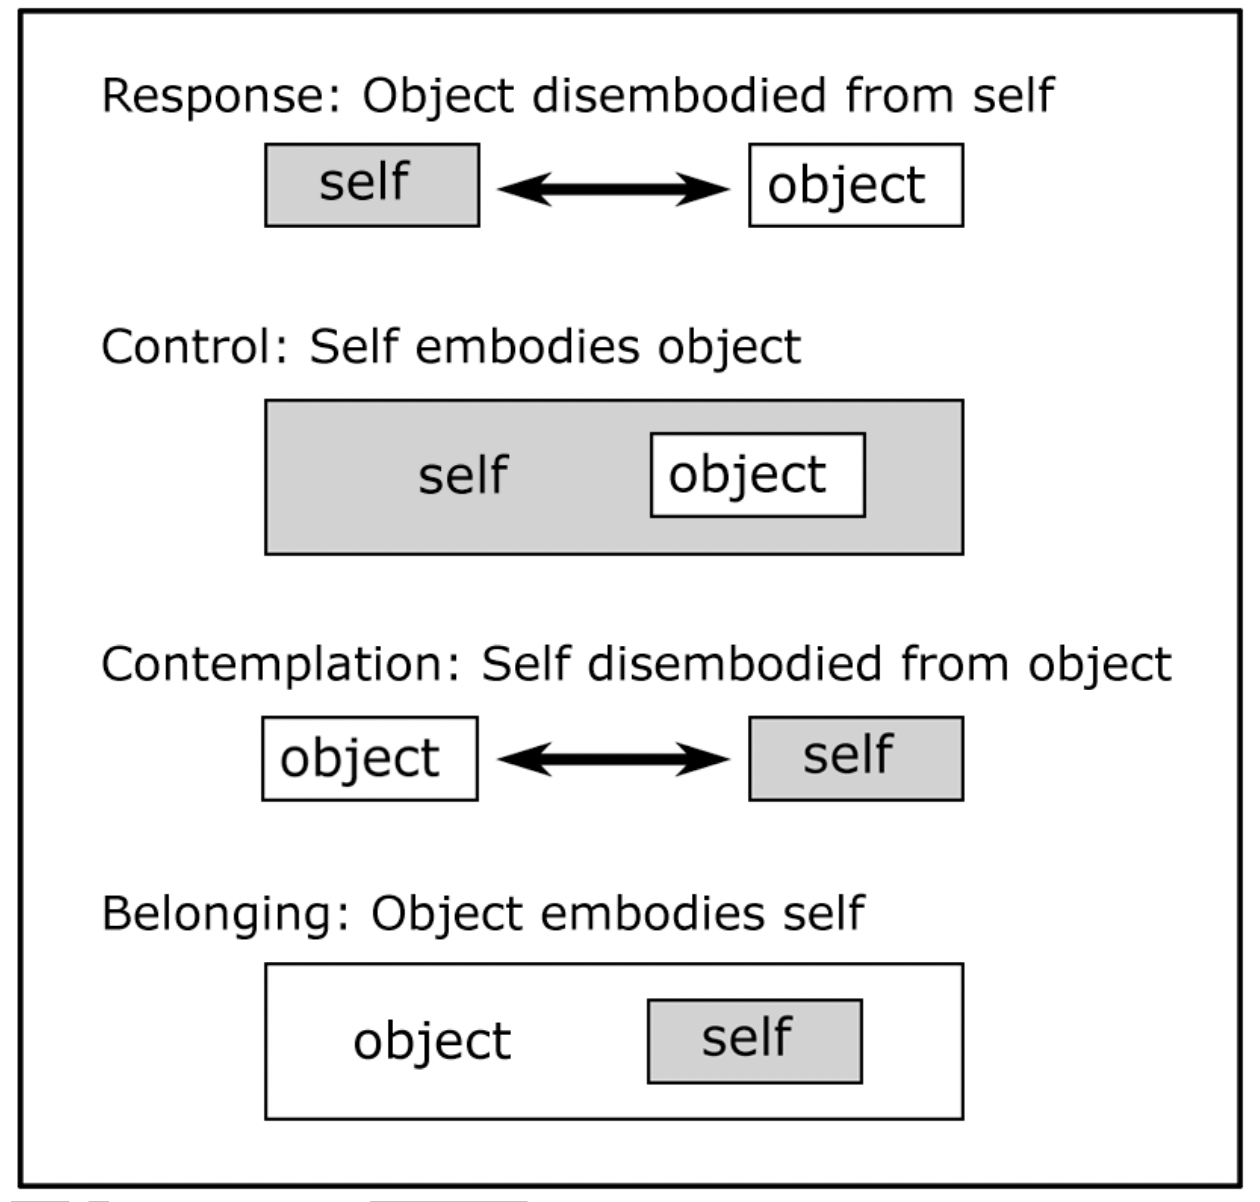
\includegraphics[width=8cm]{img/fels_diagram.png}
  \caption{Felsによるembodiment: Costelloらの論文より引用}
  \label{fig:fels_embodiment}
\end{figure}

こうしたFelsの分類は、《Iamascope》のようなインタラクティブな作品と体験者との関係を説明するために考案されたモデルであり、本研究が取り組む手指の変換という表現における、作品と体験者との関係の変化を説明する際の手段として妥当であると考えた。そのため改めて、本研究における「人馬一体」をFelsの分類から説明する。

「人馬一体」の感覚が得られるとき、人は自己に対象を帰属させている\textit{control}の関係にあるが、その過程では\textit{response}に加え、その中で対象の思い通りにいかなさや、扱いづらさなどを、対象からのメッセージとして受け止める。これはFelsのカテゴリで言えば\textit{contemplation}のカテゴリにあるといえる。さらに、そうした\textit{contemplation}を通して得られた感覚に合わせて自分の動きを変化させて応じていく様子は、Felsの分類における\textit{belonging}の関係にあると言える。

これらを踏まえると、本研究における人馬一体感とは、一体化するまでの過程で\textit{response}や\textit{contemplation}を経て、\textit{control}と\textit{belonging}が同時に起こっている状態として、説明することができる。人馬一体感をこのように捉えた上で、次章では修士作品の制作過程で行ったプロトタイピングと、「人馬一体」感の設計に向けた取捨選択について説明する。